% \documentclass[lineno,twocolumn,endfloat,biblatex]{biophys-new}
\documentclass{biophys-new}
\usepackage[utf8]{inputenc}
\usepackage{graphicx}
\usepackage[colorlinks,allcolors=cyan!70!black]{hyperref}
\usepackage{glossaries}
\usepackage{textcomp}
\usepackage{subcaption}
\usepackage{comment}
\usepackage{tikz}
\usepackage{float} 
\usepackage{datatool}
\usepackage{booktabs}
\usepackage{natbib}
\usetikzlibrary{matrix, positioning,calc,arrows.meta, backgrounds,fit}
\usepackage[dvipsnames]{xcolor}
\usetikzlibrary{shapes.geometric}
\tikzset{
    every node/.style={font=\small},
    greencycle/.style={fill=green!80!black!10,ellipse, align=center},
    rectred/.style={draw=red, fill=green!80!black!10, thick, rounded corners,  align=center},
    arrow/.style={-{Latex[length=3mm]}, thick},
}
% Uncomment if using biblatex
% \addbibresource{sample.bib}
\newacronym{nka}{NKA}{sodium-potassium ATPase pump}
\newacronym{atp}{ATP}{adenosine triphosphate}
\newacronym{adp}{ADP}{adenosine diphosphate}
\newacronym{pi}{Pi}{inorganic phosphate}
\newacronym{bcl}{BCL}{baseline cycle length}
\title{Energetic analysis of Na\textsuperscript{+}/K\textsuperscript{+}-ATPase using bond graphs}
\runningtitle{Biophysical Journal Template} %% For page header

\author[1,*]{First author}
\author[2]{Second author}
\runningauthor{Author1 and Author2} %% For page header

\affil[1]{Institution A, Address A}
\affil[2]{Institution B, Address B}

\corrauthor[*]{abx@xyz.edu}

% \papertype{Letters}
\papertype{Article}
% \papertype{Computational Tools}


\begin{document}

\begin{frontmatter}

\begin{abstract}
The sodium-potassium ATPase (NKA) consumes 19–28\% of cellular ATP and is critical for maintaining ion homeostasis. Understanding its energetic efficiency is essential for comprehending cellular physiology and pathophysiology. We develop bond graph models of the NKA that ensure thermodynamic consistency by enforcing conservation of mass, charge, and energy. A simplified 6-state model captures biophysics comparable to a 15-state model while remaining computationally tractable. Through detailed energetic analysis, we demonstrate that under physiological conditions, approximately 65\% of energy from ATP hydrolysis is stored as chemical energy in ion gradients, 10\% as electrical energy in the membrane potential, and 25\% is dissipated as heat, yielding an overall efficiency of $\sim$75\%. We investigate how the free energy of ATP hydrolysis ($\Delta G_{ATP}$), intracellular Na$^+$, and extracellular K$^+$ affect NKA efficiency and activity. A critical threshold exists at $\Delta G_{ATP} \approx -48$ kJ/mol below which chemoelectrical transduction drops dramatically, consistent with NKA inhibition under ischemic conditions. The bond graph framework enables quantitative comparison of different NKA models and provides a systematic approach for analyzing ion pumps. Energetic profiles serve as quantitative biomarkers for assessing NKA function and may inform therapeutic strategies for ion pump dysfunction in heart failure and other diseases. 
\end{abstract}

\begin{sigstatement}
The sodium-potassium ATPase is one of the body's most energy-consuming enzymes, yet its energetic efficiency and mechanisms remain incompletely understood. This study presents the first comprehensive energetic analysis using bond graph modeling, guaranteeing thermodynamic consistency. By demonstrating that simplified 6-state models capture essential energetic behaviors of complex 15-state models, we establish bond graphs as a powerful, tractable tool for energetic analysis, model comparison, model selection and validation. The bond graph approach can be applied to other transporters, offering a powerful tool for systems physiology and drug discovery.
\end{sigstatement}
\end{frontmatter}

\section*{Introduction}

The \gls{nka} is an ubiquitous enzyme that uses the energy of the hydrolysis of \gls{atp} to move Na\textsuperscript{+} ions out of the cell and K\textsuperscript{+} ions into the cell,
in both cases against steep concentration gradients. 
\Gls{atp} hydrolysis can be thought of as the energy source that tops up the cell's `sodium' battery,
since the the majority of transmembrane transport processes are driven by this sodium gradient.
The \gls{nka} is therefore critical to cellular function in all cell types and relevant to various pathophysiological conditions \cite{suhail_na_2010}.

In this paper we use a bond graph approach to examine a number of models of \gls{nka} in which mass, charge and energy are each conserved.
We examine a previously published 15-state bond graph model,
and then show how a much simpler 6-state model captures the biophysics of the pump and matches experimental data.
We then examine the energy expenditure of the \Gls{nka} and energy storage and dissipation under different conditions.
These enegergetic analyses are important to understand the efficiency of the \gls{nka} and its role in cellular energetics.
We also discuss how the energetic analysis can provide insights into the physiological function of the \gls{nka} and its implications for cellular health and disease.
We show how energetic profiles of \gls{nka} under physiological and pathophysiological conditions can be used for model validation, model comparison and model selection for different applications.

\subsection*{\Gls{nka} physiology and models}

The \Gls{nka} was discovered in 1957\cite{skou_influence_1957},
and is a chemical molecular machine responsible for the movement of Na\textsuperscript{+} and K\textsuperscript{+} ions across the cell membrane against their concentration gradients.
The Albers–Post kinetic scheme \cite{albers_role_1963,post_activation_1972} was proposed to describe the transport mechanism of the \Gls{nka} \cite{apell_electrogenic_1989},
where the \Gls{nka} undergoes Na\textsuperscript{+}-dependent phosphorylation and K\textsuperscript{+}-dependent dephosphorylation reactions and alternates between two main conformations, 
\textit{E1} and \textit{E2}, which expose the transport sites to the intracellular and extracellular sides of the membrane, respectively.

The cryo-electron microscopy (cryo-EM) structures of \Gls{nka} in different conformational states were reported,
including exoplasmic side-open (\textit{E2\textperiodcentered P})\cite{kanai_binding_2021,nguyen_structural_2022},
K\textsuperscript{+}-occluded (\textit{E2\textperiodcentered [2K] \textperiodcentered Pi}) \cite{morth_crystal_2007,shinoda_crystal_2009,nguyen_structural_2022},
(\textit{E2\textperiodcentered [2K]})\cite{guo_cryo-em_2022},
cytoplasmic side-open (\textit{E1})\cite{nguyen_structural_2022}, ATP bound cytoplasmic side-open (\textit{E1\textperiodcentered ATP})\cite{nguyen_structural_2022},
(\textit{E1\textperiodcentered [3Na]\textperiodcentered ATP})\cite{guo_cryo-em_2022}.
Na\textsuperscript{+}-occluded (\textit{E1\textperiodcentered [3Na]\textperiodcentered P\text{-}ADP}) \cite{nyblom_crystal_2013,kanai_crystal_2013,nguyen_structural_2022},
and (\textit{E1\textperiodcentered [3Na]})\cite{guo_cryo-em_2022}.
While these structural studies have provided insights into the molecular mechanism of \Gls{nka}, Wagoner et al. \cite{wagoner_mechanisms_2019} discorvered that \gls{nka} achieved high speed and efficiency by ustilizing theses multiple conformational states.

Since the \Gls{nka} transports three Na\textsuperscript{+} ions outward and two K\textsuperscript{+} ions inward,
the process gives rise to a net outward current and is therefore electrogenic \cite{apell_electrogenic_1989,glitsch_electrophysiology_2001}.
That is, the \Gls{nka} contributes to the membrane potential and the transport rate is a function of the membrane potential.
The electrogenicity of the \Gls{nka} has been studied experimentally and the main voltage-dependent steps are associated with the binding and release of Na\textsuperscript{+} ions \cite{nakao_voltage_1986,gadsby_extracellular_1993,wuddel_electrogenicity_1995,domaszewicz_binding_1999,holmgren_three_2000,holmgren_charge_2006,stanley_intracellular_2016}.
More recently, the electrogenicity of extracellular K\textsuperscript{+} binding was also investigated \cite{peluffo_electrogenic_1997,castillo_mechanism_2015}
while K\textsuperscript{+} uptake was found to be less voltage-dependent \cite{moreno_transient_2020,castillo_mechanism_2015}.

Many kinetic \Gls{nka} models, including a varied number of intermediate conformational states and partial reaction steps, have been proposed \cite{post_flexibility_1969,karlish_conformational_1978,glynn_na_1985, apell_electrogenic_1989,terkildsen_balance_2007,guerra_multistate_2025}.
Most of these models are based on the Albers-Post scheme \cite{albers_role_1963,post_activation_1972}.
Terkildsen et al. \cite{terkildsen_balance_2007} developed a kinetic model of the \Gls{nka} including fifteen intermediate states, also based on the Albers-Post scheme.
This model detailed the binding and release of Na\textsuperscript{+} and K\textsuperscript{+} ions and their voltage dependence.
It also explicitly included the proton to enable the study of the effect of pH on pump function,
which was found to be significant in ischemic conditions.
The model was subsequently corrected by Pan et al. \cite{pan_cardiac_2020} to address inconsistencies in the original model using a bond graph approach to ensure thermodynamic consistency.

The \Gls{nka} consumes 19-28\% of the total ATP consumption in mammals, and up to 50-60\% in brain and kidney \cite{rolfe_cellular_1997}.
The experimental study in guinea-pig cardiac ventricular muscle showed that the \Gls{nka} is responsible for 10\% of myocardial heat production during contraction, and 17\% at rest \cite{schramm1994energy}.
It is therefore important to guarantee thermodynamic consistency in \Gls{nka} model development. Hence, the bond graph is also used in this study, and we demonstrate how this approach facilitates energy-based analysis.

\subsection*{Bond graph in systems biology}

Bond graphs are an energy-based modelling framework originally developed in the field of engineering \cite{paynter1961analysis,karnopp2012system,breedveld1985multibond}. A comprehensive review of bond graphs in systems biology can be found in \cite{akbarpour_ghazani_review_2024}.

Gawthrop and Crampin \cite{gawthrop_energy-based_2014} pioneered the application of bond graphs to biochemical systems, demonstrating how bond graphs can ensure thermodynamic consistency in biochemical network models.
They showed that bond graphs can be used to model metabolic networks while adhering to the laws of thermodynamics, and to facilitate model reduction while preserving structural and thermodynamic properties.
The modularity of bond graphs was further explored to enable model composition with guaranteed thermodynamic consistency in \cite{gawthrop_hierarchical_2015,shahidi_hierarchical_2021,shahidi_sbml_2022,safaei_bond_2018}.
The bond graph has been extended to include chemoelectrical transduction \cite{gawthrop_bond_2017-1}, which illustrates how the energy-based approach can explicitly account for the energy flows in excitable membranes.
Pan et al. \cite{pan_bond_2018,pan_bond_2019} developed bond graph models of cardiac action potentials, demonstrating how the bond graph framework can be used to examine the conservation of physics and explain the model drift and non-unique steady states.
In \cite{gawthrop_energy-based_2017}, they domonstrated how bond graphs can facilitate analysis of energy transduction in single transporters. More complex bond graph models with feedback control have been used in \cite{gawthrop_energy-based_2021}, where the authors integrate linear control theory with bond graph modelling to analyse energy flows in biochemical networks with cyclic flow modulation.
These studies highlight the versatility and power of bond graphs in systems biology, particularly in ensuring thermodynamic consistency and facilitating energy-based analysis \cite{gawthrop_network_2022}.

\section*{Methods}
\subsection*{The bond graph modelling framework}

Bond graphs provide a useful way of formulating and visualising a thermodynamically valid biophysical model because they ensure that mass, charge and energy are each conserved, and they clearly distinguish the mechanisms for (i) transmission of power, (ii) energy storage (mechanically in a spring, electrically in a capacitor or chemically in a solute dissolved in a solvent), (iii) energy dissipation to heat (a mechanical damper, an electrical resistance or a chemical reaction), and (iv) energy transfer between mechanical, electrical or biochemical domains. Most importantly they distinguish between the conservation laws of physics and the empirically measured constitutive parameters that characterise particular materials.

In this article, we use a slightly different notation to that used in previous bond graph papers \cite{gawthrop_energy-based_2014,pan_bond_2018,pan_bond_2019,pan_cardiac_2020,hunter_energy-based_2025} to make the bond graph more accessible to a wider audience. 
We refer the reader to \cite{gawthrop_energy-based_2014,pan_bond_2018,pan_bond_2019,pan_cardiac_2020,hunter_energy-based_2025} for more details of the bond graph methodology.
Here, we only briefly introduce the key concepts of bond graph modelling relevant to this paper and explain the new notation used in the bond graph models of \Gls{nka}, as shown in in Figure~\ref{fig:bg_concepts}.
Lines of power transmission called \emph{bonds} always have an associated flux $v$ and potential $u$, and the product of flux $v$ and potential $u$ is power, i.e., $P=u\cdot v$. The arrow direction specifies the positive reference direction of the energy flow, i.e., the direction of power flow. In a dynamic system, the energy flow  $P(t)=u(t)\cdot v(t)$ direction may change over time, while a postive power $P(t)>0$ indicates the energy is released at the tail at time $t$. 

If these bonds meet, the sum of powers must be zero $\sum u\cdot v=0$, to ensure power conservation. If they share a common potential $u$ (called a \emph{0 node}), power conservation becomes just $\sum v=0$ (for non-zero u), which is mass conservation if $v$ is a molar flux or mechanical flow and charge conservation if $v$ is an electrical flux. Alternatively, if they share a common flux $v$ (called a \emph{1 node}), power conservation  becomes just $\sum u=0$ (for non-zero v), which is energy conservation.  

\begin{figure}[H]  
\centering  


% subfigures (a)--(d)

\begin{subfigure}[b]{0.2\textwidth}
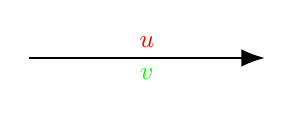
\begin{tikzpicture}
% Add an arrow from (0,0) to (3,0) and the above text at the midpoint is $u$ (in red) and below text at the midpoint is $v$( in green)
% 
    \draw[arrow] (0,0) -- (3,0) node[midway, above, red] {$u$} node[midway, below, green] {$v$};
\end{tikzpicture}
\caption{}
\end{subfigure}
\hfill
\begin{subfigure}[b]{0.2\textwidth}
% one junction- a ellipse (0:u_j^i) with five arrows pointing into it
% at the start of each arrow, only showing u_j^0, v_j^1, v_j^2, v_j^3, v_j^4, not the end of the arrow
% not showing the u_j^i at the start of each arrow
% the arrows should point towards the ellipse
% the arrows should be evenly spaced out around the ellipse
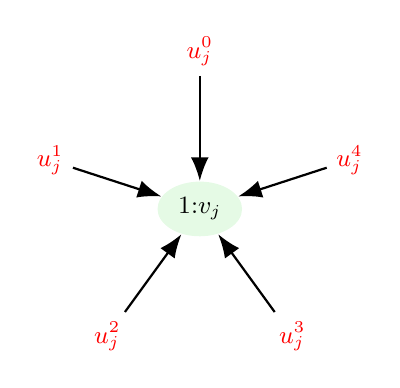
\begin{tikzpicture}
  % Arrows first, aimed at node 'zero'
  \node[greencycle, inner sep=3pt] (one) {1:$v_j$};
  \node[red](u0) at ($(one) + (90:2cm)$) {$u_j^0$};
  \node[red](u1) at ($(one) + (162:2cm)$) {$u_j^1$};
  \node[red](u2) at ($(one) + (234:2cm)$) {$u_j^2$};
  \node[red](u3) at ($(one) + (306:2cm)$) {$u_j^3$};
  \node[red](u4) at ($(one) + (18:2cm)$) {$u_j^4$};
    \draw[arrow] (u0) -- (one);
    \draw[arrow] (u1) -- (one);
    \draw[arrow] (u2) -- (one);
    \draw[arrow] (u3) -- (one);
    \draw[arrow] (u4) -- (one);
  % Node last so text is on top
\end{tikzpicture}
\caption{}
\end{subfigure}
\hfill
\begin{subfigure}[b]{0.2\textwidth}
% zero junction- a ellipse (0:u_j^i) with five arrows pointing into it
% at the start of each arrow, only showing v_j^0, v_j^1, v_j^2, v_j^3, v_j^4, not the end of the arrow
% not showing the u_j^i at the start of each arrow
% the arrows should point towards the ellipse
% the arrows should be evenly spaced out around the ellipse
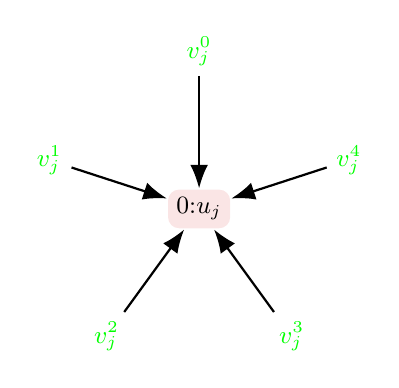
\begin{tikzpicture}
  \node[fill=red!80!black!10, thick, rounded corners, inner sep=3pt] (zero) {0:$u_j$};
  \node[green](v0) at ($(zero) + (90:2cm)$) {$v_j^0$};
  \node[green](v1) at ($(zero) + (162:2cm)$) {$v_j^1$};
  \node[green](v2) at ($(zero) + (234:2cm)$) {$v_j^2$};
  \node[green](v3) at ($(zero) + (306:2cm)$) {$v_j^3$};
  \node[green](v4) at ($(zero) + (18:2cm)$) {$v_j^4$};
    \draw[arrow] (v0) -- (zero);
    \draw[arrow] (v1) -- (zero);
    \draw[arrow] (v2) -- (zero);
    \draw[arrow] (v3) -- (zero);
    \draw[arrow] (v4) -- (zero);
  % Node last so text is on top
\end{tikzpicture}
\caption{}
\end{subfigure}
\hfill
\begin{subfigure}[b]{0.2\textwidth}
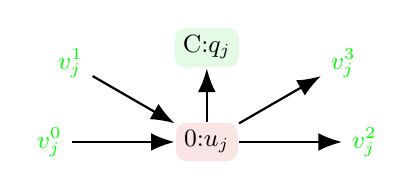
\begin{tikzpicture}[node distance=12mm ]
\node[fill=red!80!black!10, thick, rounded corners, inner sep=3pt] (zero) {0:$u_j$};
% a node above the zero node
\node[fill=green!80!black!10, thick, rounded corners, inner sep=3pt, above of=zero] (C) {C:$q_j$};
\draw[arrow] (zero) -- (C);
% two arrows pointing into the zero node from left and another two pointing out of the zero node to the right
\node[green](vL1) at ($(zero) + (180:2cm)$) {$v_j^0$};
\node[green](vL2) at ($(zero) + (150:2cm)$) {$v_j^1$};
\node[green](vR1) at ($(zero) + (0:2cm)$) {$v_j^2$};
\node[green](vR2) at ($(zero) + (30:2cm)$) {$v_j^3$};
\draw[arrow] (vL1) -- (zero);
\draw[arrow] (vL2) -- (zero);
\draw[arrow] (zero) -- (vR1);
\draw[arrow] (zero) -- (vR2);
\end{tikzpicture}
\caption{}
\end{subfigure}
\hfill
\begin{subfigure}[b]{0.2\textwidth}
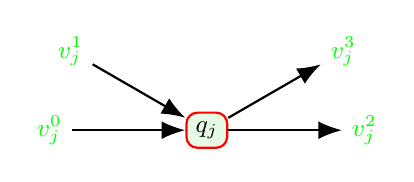
\begin{tikzpicture}[node distance=12mm ]
% node at the right of the zero and C nodes, in the middle vertically
\node[rectred] (combined) {$q_j$};
% similar layout of the arrows around the combined node
\node[green](vL1b) at ($(combined) + (180:2cm)$) {$v_j^0$};
\node[green](vL2b) at ($(combined) + (150:2 cm)$) {$v_j^1$};
\node[green](vR1b) at ($(combined) + (0:2cm)$) {$v_j^2$};
\node[green](vR2b) at ($(combined) + (30:2cm)$) {$v_j^3$};
\draw[arrow] (vL1b) -- (combined);  
\draw[arrow] (vL2b) -- (combined);
\draw[arrow] (combined) -- (vR1b);
\draw[arrow] (combined) -- (vR2b);
\end{tikzpicture}
\caption{}
\end{subfigure}


\caption{(a) a bond, which transmits energy, carries a flow $v_j$ and a potential $u_j$;
(b) a 1 node is a bond junction, where the flow is the same for all bonds and therefore the sum of potentials is zero (conservation of energy);
(c) a 0 node is a bond junction, where the potential is the same for all bonds and therefore the sum of flows is zero (conservation of mass or charge);
(d) a 0 node is usually associated with capacitive energy storage;
(e) a concise way to be more succinctly expressed by the red-bordered box where the potential $u_j$ is given by an empirically defined capacitive storage relationship $u_j=f(q_j)$.}
\label{fig:bg_concepts}
\end{figure}

The explicit expression of energy flows in bond graphs makes them particularly suitable for thermodynamic analysis of biochemical systems. For each component $j$ in the bond graph, the energy flow can be calculated as the sum of the power transmitted by each of its bonds, that is $P_j=\sum_{i = 1}^{k}  u_j^i \cdot v_j^i$ with $i=1,2,\ldots,k$ indicating the number of bonds connected to the component. For dynamic systems, the power can be integrated over time to give the total energy stored or dissipated by the component over the time interval $t_0$ to $t_1$, that is $E_j=\int_{t_0}^{t_1} P_j(t) \mathrm{d}t$.

The total energy storage and dissipation of the system can then be determined by summing the energy flows of all components. This allows for a detailed analysis of the energy budget of the system, including identifying which components are storing or dissipating the most energy, and how changes in system parameters affect the overall energy balance.

\subsection*{Bond graph models of \Gls{nka}}

\begin{figure}
\centering
\includegraphics[width=0.6\linewidth]{6state_1.pdf}
\caption{Bond graph model of \Gls{nka} with 6 states and substeps of reaction. (1) The enzyme ($E_i$) binds three intracellular Na\textsuperscript{+} ions from the cytoplasm and ATP binds to the enzyme-3Na\textsuperscript{+} complex, leading to ($E_i\cdot ATP \cdot 3Na^+$); (2) The enzyme-3Na\textsuperscript{+}-ATP complex undergoes phosphorylation and ADP is released, leading to the formation of the enzyme-3Na\textsuperscript{+}-P complex ($E_i\cdot P_i \cdot 3Na^+$); (3) The enzyme-3Na\textsuperscript{+}-P complex undergoes a conformational change to the exoplasmic side-open state, releasing three Na\textsuperscript{+} ions to the extracellular space ($E_o\cdot P_i$); (4) Two extracellular K\textsuperscript{+} ions bind to the enzyme in the exoplasmic side-open state, leading to enzyme-2K\textsuperscript{+} complex ($E_o\cdot P_i \cdot 2K^+$); (5) The enzyme-2K\textsuperscript{+} complex ($E_o\cdot P_i \cdot 2K^+$) undergoes dephosphorylation, releasing $P_i$ and $H^+$, ending up with the enzyme-2K\textsuperscript{+} complex ($E_o\cdot 2K^+$); (6) The enzyme-2K\textsuperscript{+} complex ($E_o\cdot 2K^+$) undergoes a conformational change to the cytoplasmic side-open state ($E_i$), leading to the release of two K\textsuperscript{+} ions into the cytoplasm.}
\label{fig:6state_v1}
\end{figure}

We here explain the construction of 6-state bond graph model of \Gls{nka} using the new notation,
while the 15-state model is explained in \cite{pan_cardiac_2020} and the graph using the new notation is in the supplementary material.
The bond graph mode of \Gls{nka} with 6 states is based on the scheme proposed in Fig. 1b of \cite{nguyen_structural_2022} with slight modifications.
We merged (\textit{E1\textperiodcentered [3Na]\textperiodcentered ATP}) and (\textit{E1\textperiodcentered [3Na]\textperiodcentered P\text{-}ADP}), 
while splitting the release of \gls{adp} and Na\textsuperscript{+} into two steps. The graphic representation of the model is shown in Figure \ref{fig:6state_v1} with the steps of the transporters, where we label the cytoplasmic side-open state (\textit{E1}) as $E_i$  and the exoplasmic side-open state \textit{E2} as $E_o$. We also derived the analytical steady state equations of this model in the supplementary material, which will be used to check when the instantaneous dynamics of the model differ from the steady state. 

\subsection*{Energetic analysis of \gls{nka} models}

The \gls{nka} extrudes three Na\textsuperscript{+} ions from the intracellular space and imports two K\textsuperscript{+} ions into the cell per molecule of \gls{atp} hydrolyzed. The overall reaction can be summarised as:
\begin{equation}
      \label{eq:nka_reaction}
      ATP + 3Na^+_i + 2K^+_o \rightarrow ADP + P_i + 3Na^+_o + 2K^+_i + H^+
\end{equation}
where the subscripts $i$ and $o$ denote intracellular and extracellular species, respectively.

The energy released from \gls{atp} hydrolysis is used to drive the transport of Na\textsuperscript{+} and K\textsuperscript{+} ions against their electrochemical gradients. The Gibbs free energy change associated with \gls{atp} hydrolysis can be expressed as:
\begin{equation}
      \label{eq:atp_hydrolysis}
      \Delta G_{ATP} =  u_{ADP} + u_{P_i} + u_{H^+} - u_{ATP}
\end{equation}
where $u_{ATP}$, $u_{ADP}$, $u_{P_i}$, and $u_{H^+}$ are the chemical potentials of \gls{atp}, \gls{adp}, \gls{pi}, and protons $H^+$, respectively.

The thermodynamic efficiency of the \gls{nka} at steady state can be estimated using Equation \ref{eq:efficiency_estimate} \cite{wagoner_mechanisms_2019} below:
\begin{equation}
      \label{eq:efficiency_estimate}
      \eta_{est} = \frac{\left(3u_o^{Na^+} + 2u_i^{K^+}-3u_i^{Na^+}-2u_o^{K^+}-FV_m\right)}{\Delta G_{ATP}} \cdot 100\%
\end{equation}

where $u_i^{Na+}$ and $u_o^{Na+}$ are the chemical potentials of intracellular and extracellular Na\textsuperscript{+}, respectively,
$u_i^{K+}$ and $u_o^{K+}$ are the chemical potentials of intracellular and extracellular K\textsuperscript{+}, respectively,
$F$ is Faraday's constant, and $V_m$ is the membrane potential.

Under physiological conditions, the membrane potential, particularly for cardiac cells, varies over time and the variation affects the thermodynamic efficiency of the \gls{nka} \cite{wagoner_mechanisms_2019,peluffo_nak-atpase_2023}. 

The energy flows in the \gls{nka} are shown in Figure \ref{fig:NKA}. ATP hydrolysis release energy to drive the transport of Na\textsuperscript{+} and K\textsuperscript{+} ions. Some energy is dissipated as heat, while the rest is stored as chemical energy in the concentration gradients of Na\textsuperscript{+} and K\textsuperscript{+} across the cell membrane and electrical energy in the membrane potential.

\begin{figure}
\centering


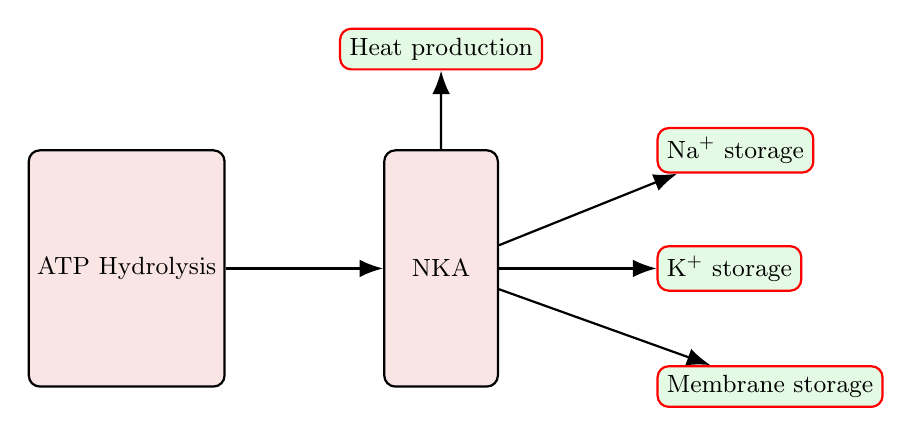
\begin{tikzpicture}[scale=0.75]
% Add an arrow from (0,0) to (3,0) and the above text at the midpoint is $\mu$ (in red) and below text at the midpoint is $v$( in green)
   \node[draw=black,fill=red!80!black!10, thick, rounded corners, inner sep=3pt,minimum height=3cm] (atp) {ATP Hydrolysis};
   \node[draw=black,fill=red!80!black!10, thick, rounded corners, inner sep=10pt, minimum height=3cm, right=2cm of atp] (nka) {NKA};
% nodes Na^+ storage, K^+ storage, membrane storage, heat production at the right of nka evenly spaced out in vertically
   \node[rectred, right=2cm of nka, yshift=1.5cm] (Na_i) {Na$^+$ storage};
   \node[rectred, right=2cm of nka, yshift=0cm] (K_i) {K$^+$ storage};
   \node[rectred, right=2cm of nka, yshift=-1.5cm] (mem) {Membrane storage};
   \node[rectred, above=1cm of nka] (heat) {Heat production};
   \draw[arrow] (atp) -- (nka);
   \draw[arrow] (nka) -- (Na_i);
   \draw[arrow] (nka) -- (K_i);
   \draw[arrow] (nka) -- (mem);
   \draw[arrow] (nka) -- (heat);
\end{tikzpicture}




\caption{Schematic diagram of energy flows through the \gls{nka}.}
\label{fig:NKA}
\end{figure}

In this study, we perform a detailed energetic analysis of the \gls{nka} models using the bond graph framework to account for the time-varying nature of the membrane potential and other dynamic factors. The total energy supplied by \gls{atp} hydrolysis over a time interval $t$ can be calculated as:
\begin{equation}
      \label{eq:energy_supply}
      E_{supply} = \int_{0}^{t} u_{ATP} \cdot v_{ATP} \mathrm{d}t- \int_{0}^{t} u_{ADP} \cdot v_{ADP} \mathrm{d}t - \int_{0}^{t} u_{P_i} \cdot v_{P_i} \mathrm{d}t - \int_{0}^{t} u_{H^+} \cdot v_{H^+} \mathrm{d}t
\end{equation}

where $v_{ATP}$, $v_{ADP}$, $v_{P_i}$, and $v_{H^+}$ are the flow rates of \gls{atp} hydrolysis, \gls{adp} production, \gls{pi} production, and proton production, respectively. 

The energy dissipated by the \gls{nka} depends on the model structure, and can be calculated as:
\begin{equation}
      \label{eq:energy_dissipation}
      E_{dissipation} = \sum_{i = 1}^{k} \int_{0}^{t} \left(A^f_{i}-A^r_{i}\right) \cdot v_{i} \mathrm{d}t
\end{equation}

where $A^f_{i}$ and $A^r_{i}$ are the forward and reverse affinities of reaction $i$, respectively, $v_{i}$ is the flow rate of reaction $i$, and $k$ is the total number of reactions in the \gls{nka} models. For 15-state model, $k = 15$, and for 6-state model, $k = 6$.

 The chemical energy stored in the concentration gradients of Na\textsuperscript{+} and K\textsuperscript{+} concentration gradients across the cell membrane can be calculated as:
\begin{equation}
      \label{eq:energy_storage_Na}
      E_{storage}^{Na^+} = \int_{0}^{t}u_o^{Na+} \cdot v_o^{Na+} \mathrm{d}t- \int_{0}^{t} u_i^{Na+} \cdot v_i^{Na+}  \mathrm{d}t 
\end{equation}
\begin{equation}
      \label{eq:energy_storage_K}
      E_{storage}^{K^+} =  \int_{0}^{t}u_i^{K+} \cdot v_i^{K+} \mathrm{d}t- \int_{0}^{t} u_o^{K+} \cdot v_o^{K+}  \mathrm{d}t 
\end{equation}
where $v_i^{Na+}$ and $v_o^{Na+}$ are the flow rates of intracellular and extracellular Na\textsuperscript{+}, respectively;
$v_i^{K+}$ and $v_o^{K+}$ are the flow rates of intracellular and extracellular K\textsuperscript{+}, respectively.

The total stored chemical energy can then be calculated as:
\begin{equation}
      \label{eq:total_energy_storage}
      E_{storage}^{chemical} = E_{storage}^{Na^+} + E_{storage}^{K^+}
\end{equation}

The electrical energy stored in the membrane potential can be calculated as:
\begin{equation}  
      \label{eq:electrical_energy}
      E_{storage}^{electrical} = \int_{0}^{t} u_m^e \cdot v_m^e \mathrm{d}t
\end{equation}
where $V_m$ is the membrane potential and $i_{m}$ is the current mediated by the \gls{nka}.

The total energy balance of the \gls{nka} model can be written as:
\begin{equation}
      \label{eq:total_energy_balance}
      E_{total} = E_{supply} - E_{dissipation} - E_{storage}^{chemical} - E_{storage}^{electrical}
\end{equation}
where $E_{total}$ should be zero to satisfy the first law of thermodynamics.

The thermodynamic efficiency of the \gls{nka} can be defined as the ratio of the useful energy stored to the total energy supplied:
\begin{equation}
      \label{eq:efficiency}
      \eta = \frac{E_{storage}^{chemical} + E_{storage}^{electrical}}{E_{supply}}\cdot 100\%
\end{equation}

The chemical energy conversion efficiency of the \gls{nka} can be defined as the ratio of chemical energy stored to the total energy supplied:
\begin{equation}
      \label{eq:chemical_efficiency}
      \eta_{ch} = \frac{E_{storage}^{chemical}}{E_{supply}}\cdot 100\%
\end{equation}
The electrical energy conversion efficiency of the \gls{nka} can be defined as the ratio of electrical energy stored to the total energy supplied:
\begin{equation}
      \label{eq:electrical_efficiency}
      \eta_{e} = \frac{E_{storage}^{electrical}}{E_{supply}}\cdot 100\%
\end{equation}

The ratio of heat production (i.e. energy dissipation) also be calculated to assess the energy loss in the \gls{nka}:
\begin{equation}
      \label{eq:energy_loss}
      \lambda = \frac{E_{dissipation}}{E_{supply}}
\end{equation}

The ratio of chemical energy stored to electrical energy stored can be calculated to assess the distribution of energy storage in the \gls{nka}:
\begin{equation}
      \label{eq:energy_distribution}
      \gamma = \frac{E_{storage}^{chemical}}{E_{storage}^{electrical}}
\end{equation}
\subsection*{Simulation conditions}

In this paper, we focus on the energetic analysis of \gls{nka} under physiological conditions, and we set up the simulation conditions based on the literature review as follows.
Since \gls{atp} hydrolysis serves as the energy source for the \gls{nka}, the free energy change of \gls{atp} hydrolysis ($\Delta G_{ATP}$) plays a crucial role in determining the activity of the \gls{nka}.
The $\Delta G_{ATP}$ depends on the concentrations of \gls{atp}, \gls{adp}, \gls{pi}, and $H^+$ (i.e, pH value).

The intracellular\gls{atp} concentration ranges from 1.92–7.47 $mM$ with average of 4.4 $mM$ \cite{greiner_intracellular_2021},
while the recent study showed lower diastolic cytosolic \gls{atp} levels around 457 $\pm 47u M$ (less than 1 mM), which is less than previously estimated, and fluctuations during excitation-contraction coupling \cite{rhana_fueling_2024}.

The cytosolic \gls{adp} concentrations of in situ mouse, rat and guinea pig heart are 13, 18 and 22 $u M$ \cite{dobson_heart_2002}, respectively, while the extrapolated value in human heart is 45.66 $u M$  with 70 kg body weight.
The experimental observation of \gls{pi} in the heart in vivo has not been studied yet, while the baseline \gls{pi} of a model prediction in the canine myocyte cytoplasm is around 0.29 mM and increases with work rate in heart cells \cite{wu_phosphate_2008}.


The model simulation \cite{tran_regulation_2015} reported \gls{atp}, \gls{adp}, \gls{pi} and pH values of 5.61 mM, 25.4 $u M$, 1.16 mM and 7.15, respectively. In general, the physiological intracellular pH ranges from 7.15 to 7.25 \cite{orlowski_intracellular_2025}

Intracellular Na\textsuperscript{+} concentration is normally from 4 to 16 mM \cite{bers_intracellular_2003}, while the level can rise by 3 mM above this value in heart failure conditions \cite{despa_intracellular_2002}. This increase was due to increased Na\textsuperscript{+} influx while the \gls{nka} function is unchanged \cite{despa_intracellular_2002}.
Around 98 \% potassium (K\textsuperscript{+}) resides in the cytosol at 140-150 mM and the extracellular K\textsuperscript{+} concentration ranges from 3.5 to 5 mM \cite{zacchia_potassium_2016}.

We use the simulation conditions as shown in Table \ref{tab:default_parameters} to examine the distribution of energy flows in different \gls{nka} models. In addition, we vary one parameter at a time to investigate its effect on the function and energetics of the \gls{nka} and varied values are shown in the results section.

\begin{table}[htbp]
\centering
\DTLloaddb[
  keys={Parameter,Description,Value,Units,References}
]{mydata}{default_conditions.csv}
\begin{tabular}{lllll}
\toprule
Parameter & Description & Value & Units & References\\
\midrule
\DTLforeach{mydata}{%
  \param=Parameter,\desc=Description,\val=Value,\unit=Units,\refs=References%
}{%
  \param & \desc & \val & \unit & \citep{\refs}\\
}
\end{tabular}
\caption{Default parameters for \gls{nka}.}
\label{tab:default_parameters}
\end{table}

\section*{Results}
\subsection*{Fit 6-state \gls{nka} models to experimental data}
We applied the experimental conditions in \cite{pan_cardiac_2020} to fit the 6-state bond graph model to the experimental data, shown in Figure \ref{fig:model_fit}. 

\begin{figure}[htbp]
\centering
\begin{subfigure}{0.35\textwidth}
      \centering
      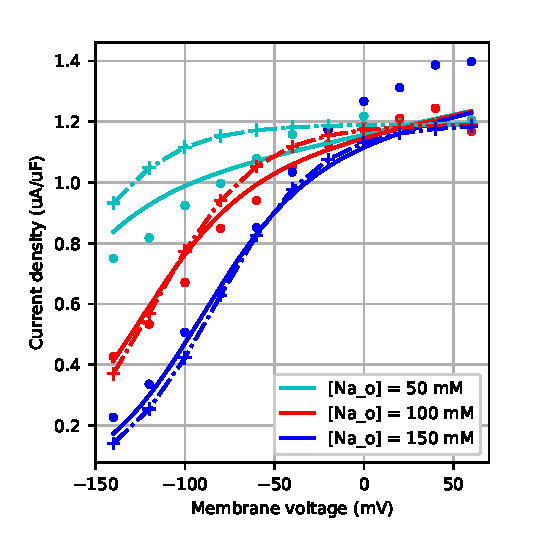
\includegraphics[width=\linewidth]{figures/NKE_BG_6_state_fig2b_fit.eps}
      \caption{Data from Figure 2b in \cite{pan_cardiac_2020}}
\end{subfigure}
\begin{subfigure}{0.35\textwidth}
      \centering
      \includegraphics[width=\linewidth]{figures/NKE_BG_6_state_fig3a_fit.eps}
      \caption{Data from Figure 3a in \cite{pan_cardiac_2020}}
\end{subfigure}
\begin{subfigure}{0.35\textwidth}
      \centering
      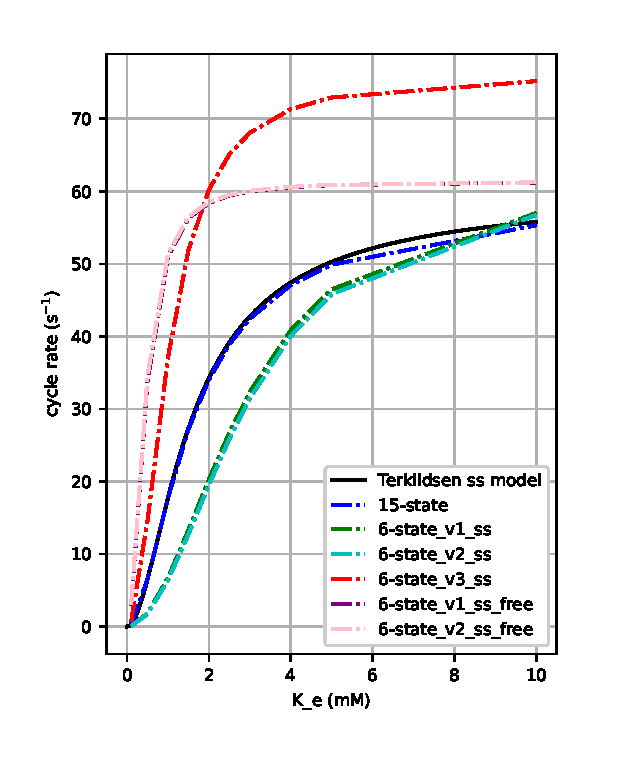
\includegraphics[width=\linewidth]{figures/NKE_BG_6_state_fig3b_fit.eps}
      \caption{Data from Figure 3b in \cite{pan_cardiac_2020}}
\end{subfigure}
\begin{subfigure}{0.35\textwidth}
      \centering
      \includegraphics[width=\linewidth]{figures/NKE_BG_6_state_fig3c_fit.eps}
      \caption{Data from Figure 3c in \cite{pan_cardiac_2020}}
\end{subfigure}
\caption{Fit of \gls{nka} models to experimental data and Terkildsen model after correction in \cite{pan_cardiac_2020}. The solid lines are simulated data from the kinetic model in \cite{pan_cardiac_2020}, while the solid dots are experimental data. The dashed lines are simulated data from the steady-state 6-state bond graph model, and the '+' symbols are produced by the full 6-state bond graph model. (a) \gls{nka} current-voltage relationship at different extracellular Na\textsuperscript{+} concentrations; (b) \gls{nka} current as a function of intracellular Na\textsuperscript{+} concentration; (c) \gls{nka} current as a function of extracellular K\textsuperscript{+} concentration;  (d) \gls{nka} current as a function of ATP concentration. The simulation conditions are the same as in \cite{pan_cardiac_2020}.}
\label{fig:model_fit} 
\end{figure}

The simulated data are comparable to the kinetic model in \cite{pan_cardiac_2020} and experimental data under most conditions, except for the low extracellular Na\textsuperscript{+} concentration (50 mM) in Figure \ref{fig:model_fit} (a).
The 6-state model has higher current density when the extracellular Na\textsuperscript{+} concentration is 50 mM compared to the kinetic model in \cite{pan_cardiac_2020}, while extracellular Na\textsuperscript{+} concentration is normally around 140 mM \cite{bers_intracellular_2003} under physiological conditions.
In the following sections, we will focus on the comparison of the 15-state and 6-state bond graph models with regard to thermodynamic aspects, which is the main focus of this study.

\subsection*{Energy flows through \gls{nka}}

We applied a series of action potentials (with \gls{bcl} of 1000 ms) to the \gls {nka} models. The action potentials were simulated using the Faber-Ludy model\cite{faber_action_2000} with corrected T type calcium current \cite{tong_computational_2014} , which were retrieved from PMR (\url{https://models.physiomeproject.org/e/260}). The other simulation conditions are shown in Table \ref{tab:default_parameters}. We then calculated the energy flows through the \gls{nka} over six cycles of the action potential. We plot the results in Figure \ref{fig:energy_flow} (a and b). 

\begin{figure}[htbp]
\centering
\begin{subfigure}{0.4\textwidth}
      \centering
      \includegraphics[width=\linewidth]{figures/EA_report_task_NKE_BG_15_state_default_Sankey.png}
      \caption{15-state model}
\end{subfigure}
\begin{subfigure}{0.4\textwidth}
      \centering
      \includegraphics[width=\linewidth]{figures/EA_report_task_NKE_BG_6_state_ATPNaZK_free_default_Sankey.png}
      \caption{6-state model}
\end{subfigure}
\begin{subfigure}{0.6\textwidth}
      \centering
      \includegraphics[width=\linewidth]{figures/EA_15state_heat_bar.png}
      \caption{15-state model}
\end{subfigure}
\begin{subfigure}{0.3\textwidth}
      \centering
      \includegraphics[width=\linewidth]{figures/EA_6state_heat_bar.png}
      \caption{6-state model}
\end{subfigure}
\caption{Energy flow diagrams and heat production rates of (a) 15-state model and (b) 6-state model of \gls{nka} under physiological conditions.}
\label{fig:energy_flow} 
\end{figure}

We can see that around 25\% of the energy supplied by ATP hydrolysis is dissipated as heat, 10\% is stored as electrical energy, and 65\% is stored as chemical energy in both models under physiological conditions. The thermodynamic efficiency of both models is around 75\%, which is consistent with previous theoretical studies \cite{wagoner_mechanisms_2019,peluffo_nak-atpase_2023}.
We also calculated the heat production rates of both models, shown in Figure \ref{fig:energy_flow} (c and d).
In 15-state model, the energy dissipation mainly occurs during the reaction steps of $Rx_m^6$ when \gls{adp} is released, and $Rx_m^{13}$ when $P_i$ and $H^+$ are released and $Rx_m^{15}$ when the enzyme is translocated from extracellular to intracellular after \gls{atp} binding.
In 6-state model, the energy dissipation mainly occurs during the reaction steps of $Rx_m^2$ when \gls{adp} is released, and $Rx_m^{5}$ when $P_i$ and $H^+$ are released.

According to the theoretical study in \cite{wagoner_mechanisms_2019}, the \gls{nka} is a highly efficient molecular machine due to the micro conformational changes that minimize energy loss during ion transport. The data in their study showed that the efficiency of \gls{nka} ranges from around 50\% to 88\% depending on operating conditions.

Another theoretical study in \cite{peluffo_nak-atpase_2023} speculated that the ratio of Na\textsuperscript{+} to K\textsuperscript{+} transport is optimized to achieve maximum efficiency, cell volume homeostasis, and stable electrochemical gradients. 

In the following section, we will further investigate the thermodynamic efficiency of the \gls{nka} under a range of conditions, which provides insights into the energy transduction mechanisms of the \gls{nka}. With this understanding, scientists can better select appropriate \gls{nka} models for their research and develop more accurate models in the future.

\subsection*{Thermodynamic efficiency of \Gls{nka} }


To investigate the thermodynamic efficiency of the \gls{nka} under physiological conditions, we applied the action potential with different \gls{bcl} to simulate the \gls{nka} models, and calculated the thermodynamic efficiency over one six cycles.
We also vary the \gls{atp}, \gls{adp}, \gls{pi} concentrations and pH values to examine their effects on the thermodynamic efficiency of the \gls{nka}.
When varying one parameter, the other parameters are set to the default values in Table \ref{tab:default_parameters}.
The corresponding $\Delta G_{ATP}$ values range from -46 kJ/mol to -62 kJ/mol, indicated by the blue dots in the plots, shown in Figure \ref{fig:thermodynamic_efficiency_AP}.

\begin{figure}[htbp]
\centering
\begin{subfigure}{0.48\textwidth}
      \centering
      \includegraphics[width=\linewidth]{figures/EA_2D_combine_15state_Thermodynamic_efficiency.png}  
      \caption{15-state model}    
\end{subfigure}
\hfill
\begin{subfigure}{0.48\textwidth}
      \centering  
      \includegraphics[width=\linewidth]{figures/EA_2D_combine_6state_Thermodynamic_efficiency.png}
      \caption{6-state model}    
\end{subfigure}
\caption{Thermodynamic efficiency of \gls{nka} (a) (15-state model) and (b) (6-state model). The right y-axis shows the corresponding $\Delta G_{ATP}$ values, indicated by the blue dots in the plots.}
\label{fig:thermodynamic_efficiency_AP} 
\end{figure} 

With increased \gls{atp} concentrations, the thermodynamic efficiency of both models rapidly increases intially and then drops to a relatively stable level around 70\%.
The 15-state model has slightly higher efficiency than the 6-state model at most \gls{atp} concentrations, which is consistent with the theoretical study in \cite{wagoner_mechanisms_2019} that more substeps in the transport cycle lead to higher efficiency.

With increased \gls{adp} concentrations and \gls{pi} concentrations, the thermodynamic efficiency of both models increases rapidly at low concentrations and then reaches a plateau. Afterward, the full bond graph models present a decrease in efficiency at high concentrations, while the steady-state models maintains relatively stable efficiency.
The study \cite{wu_phosphate_2008} showed the free \gls{adp} slightly increases from 0.042 mM to 0.064 mM , while the \gls{pi} concentration is approximately 0.29 mM and increases to 2.3 mM at high work rate. According to our simulation, the increased \gls{adp} and \gls{pi} concentrations during high work rate will make the \gls{nka} operate at a higher efficiency.

In majority of the pH range (5.5-8), the thermodynamic efficiency of both models decreases linearly with increased pH values. 

From the figures, we can see that the \gls{atp}, \gls{adp}, \gls{pi} concentrations and pH values affect the thermodynamic efficiency of \gls{nka} in a different manner even though the $\Delta G_{ATP}$ values are within same range. To further investigate the effect of $\Delta G_{ATP}$ on the thermodynamic efficiency of \gls{nka}, we plotted the thermodynamic efficiency of both models under different $\Delta G_{ATP}$ values by varying the \gls{atp}, \gls{adp}, \gls{pi} concentrations and pH values, shown in Figure \ref{fig:thermodynamic_efficiency_AP_deltaGATP}. 

\begin{figure}[htbp]
\centering
\begin{subfigure}{0.4\textwidth}
      \centering
      \includegraphics[width=\linewidth]{figures/EA_2D_combine_15state_Thermodynamic_efficiency_deltaATP.png}  
      \caption{15-state model}    
\end{subfigure}
\begin{subfigure}{0.4\textwidth}
      \centering  
      \includegraphics[width=\linewidth]{figures/EA_2D_combine_6state_Thermodynamic_efficiency_deltaATP.png}
      \caption{6-state model}    
\end{subfigure}
\caption{Thermodynamic efficiency of \gls{nka} (a) (15-state model) and (b) (6-state model) under different $\Delta G_{ATP}$ values.}
\label{fig:thermodynamic_efficiency_AP_deltaGATP} 
\end{figure}

We can see that the thermodynamic efficiency of both models increases with lower $\Delta G_{ATP}$ values (less negative), and there is a drop in full bond graph models after the $\Delta G_{ATP}$ reaches around -48 kJ/mol. This seems alighned with the study \cite{kammermeier_high_1987,glitsch_change_1995}. Kammermeier estimated that the \gls{nka} in the heart requires a minimum $\Delta G_{ATP}$ of $-46~kJ/mol$, while the study \cite{glitsch_change_1995} found that when $\Delta G_{ATP}$ was approximately $-49~kJ/mol$, little activity of \gls{nka} at membrane potentials more negative than $-75~mV$ was observed in sheep Purkinje cells.

To investigate the meachinisim behind the drop in thermodynamic efficiency at low $\Delta G_{ATP}$ values, we computed biochemical conversions efficiency $\eta_{ch}$ and electrical conversion efficiency $\eta_{e}$ using equations \ref{eq:chemical_efficiency} and \ref{eq:electrical_efficiency}, respectively.
We found out that the drop mainly due to decreased electrical conversion efficiency, as shown in Figure \ref{fig:electrical_efficiency_AP_deltaGATP}.

\begin{figure}[htbp]
\centering
\begin{subfigure}{0.4\textwidth}
      \centering
      \includegraphics[width=\linewidth]{figures/EA_2D_combine_15state_Electrical_conversion_efficiency_deltaATP.png}  
      \caption{15-state model}    
\end{subfigure}
\begin{subfigure}{0.4\textwidth}
      \centering  
      \includegraphics[width=\linewidth]{figures/EA_2D_combine_6state_Electrical_conversion_efficiency_deltaATP.png}
      \caption{6-state model}    
\end{subfigure}
\caption{Electrical conversion efficiency of \gls{nka} (a) (15-state model) and (b) (6-state model) under different $\Delta G_{ATP}$ values.}
\label{fig:electrical_efficiency_AP_deltaGATP} 
\end{figure}

We can see that the electrical conversion efficiency of both models slightly increases with lower $\Delta G_{ATP}$ values (less negative), and there is a drop to negative in full bond graph models after the $\Delta G_{ATP}$ reaches around -48 kJ/mol, which aligns with the drop in thermodynamic efficiency. 

The trends of the electrical conversion efficiency of both models are similar under varying \gls{atp}, \gls{pi} concentrations, but different with varied  \gls{adp} and pH values.
With varied \gls{adp}, the electrical conversion efficiency of 6-state model starts to decrease earlier than the 15-state model;
with varied pH, the electrical conversion efficiency of 15-state steady-state model does not drop at all.
Theese differences may be due to the different confirguration of multiple reaction steps of the two models.


Under physiological conditions, the current mediated by the \gls{nka} is outward.
When the free energy available from ATP hydrolysis ($\Delta G_{ATP}$) decreases (less negative), the current reduces and eventually reverses direction, leading to an inward current, as observed experimentally in \cite{glitsch_change_1995}.
In our simulation, the energy flow (i.e., power output) of the membrane potential becomes negative when \gls{pi} or \gls{adp} concentration is increased, or pH is decreased,
which means that the charges over the membrane act as energy source.
This leads to a drop in electrical conversion efficiency and consequently a drop in thermodynamic efficiency of the \gls{nka}.

It is worth noting that the electrical conversion efficiency is lower at higher work rate (i.e. shorter \gls{bcl}).

\subsection*{Inhibition of \Gls{nka} by reduced \texorpdfstring{$\Delta G_{ATP}$}{Lg}}

Jansen et al. \cite{jansen2003energy} investigated the effect of reduced free energy available from ATP hydrolysis on \gls{nka} activity in oxygenated isolated rat heart. 
In their study, they cannot distinguish whether the effect on \gls{nka} activity was due to changes in ATP, ADP, Pi, or pH, but they observed that as $\Delta G_{ATP}$ decreased, there was a reduction in $Rb^+$ uptake, indicating reduced \gls{nka} activity.

We ploted the mean turnover rate of \gls{nka} under different $\Delta G_{ATP}$ values by varying the \gls{atp}, \gls{adp}, \gls{pi} concentrations and pH values, shown in Figure \ref{fig:Mean_flow_rate_AP_deltaGATP}. 

\begin{figure}[htbp]
\centering
\begin{subfigure}{0.4\textwidth}
      \centering
      \includegraphics[width=\linewidth]{figures/EA_2D_combine_15state_Mean_flow_rate_deltaATP.png}  
      \caption{15-state model}    
\end{subfigure}
\begin{subfigure}{0.4\textwidth}
      \centering  
      \includegraphics[width=\linewidth]{figures/EA_2D_combine_6state_Mean_flow_rate_deltaATP.png}
      \caption{6-state model}    
\end{subfigure}
\caption{Mean flow rate of \gls{nka} (a) (15-state model) and (b) (6-state model) under different $\Delta G_{ATP}$ values.}
\label{fig:Mean_flow_rate_AP_deltaGATP} 
\end{figure}

We can see that the mean turnover rate of both models decreases with lower $\Delta G_{ATP}$ values (less negative), which aligns with the experimental observation in \cite{jansen2003energy}.

Huang et al. \cite{huang1984regulation} found that the inhibition of \gls{nka} activity by \gls{pi} depended on the pH range, with greater inhibition at lower pH values of 6.1 -7, but less inhibition with increased pH of 7 - 8.5. With 5 mM \gls{pi}, the \gls{nka} activity was inhibited by around 30\% at pH 7.
In our simulation, we can see that the inhibition of \gls{nka} activity by \gls{pi} is more pronounced at lower $\Delta G_{ATP}$ values, which is associated with lower pH values and higher \gls{pi} concentrations.

Increase in intracellular \gls{pi} and decreases in intracellular pH and ATP were associated with ischemic conditions \cite{huang1984regulation,wu_phosphate_2008}, and these changes are associated with the inhibition of \gls{nka} activity if other conditions are kept constant according to our simulation.

To understand how the inhibition of \gls{nka} activity affects its thermodynamic efficiency, we plotted the thermodynamic efficiency of both models under different mean turnover rates by varying the \gls{atp}, \gls{adp}, \gls{pi} concentrations and pH values, shown in Figure \ref{fig:thermodynamic_efficiency_AP_flowRate}.

\begin{figure}[htbp]
\centering
\begin{subfigure}{0.4\textwidth}
      \centering
      \includegraphics[width=\linewidth]{figures/EA_2D_combine_15state_Thermodynamic_efficiency_flowRate.png}  
      \caption{15-state model}    
\end{subfigure}
\begin{subfigure}{0.4\textwidth}
      \centering  
      \includegraphics[width=\linewidth]{figures/EA_2D_combine_6state_Thermodynamic_efficiency_flowRate.png}
      \caption{6-state model}    
\end{subfigure}
\caption{Thermodynamic efficiency of \gls{nka} (a) (15-state model) and (b) (6-state model) under different mean turnover rates.}
\label{fig:thermodynamic_efficiency_AP_flowRate} 
\end{figure}

We can see that the thermodynamic efficiency of both models increases with reduced mean turnover rates, which aligns with the study in \cite{wagoner_mechanisms_2019}.
The drop in thermodynamic efficiency at very low mean turnover rates in full bond graph models is due to the drop in electrical conversion efficiency, as discussed in the previous section.


\subsection*{Response of \Gls{nka} to changes in intracellular \texorpdfstring{Na\textsuperscript{+}}{Lg} concentration and extracellular \texorpdfstring{K\textsuperscript{+}}{Lg} concentration}

The reduction of free energy available from ATP hydrolysis results in an accumulation of intracellular Na\textsuperscript{+} ions \cite{jansen2003energy}.
The increase was noted when $\Delta G_{ATP}$ fell below $-52~kJ/mol$ and larger increases were noted when $\Delta G_{ATP}$ dropped below $-48~kJ/mol$.
This finding agreed with the experimental observation that little activity of of \gls{nka} at membrane potentials more negative than $-75~mV$ was observed when $\Delta G_{ATP}$ was approximately $-49~kJ/mol$ \cite{glitsch_change_1995}.
These observations are consistent with our simulation results, shown in Figure \ref{fig:Mean_flow_rate_AP_deltaGATP}, where the decrease in mean turnover rate of both models are more significant at lower $\Delta G_{ATP}$ values (less negative).

Despa et al. \cite{despa_intracellular_2002} reported that the resting intracellular Na\textsuperscript{+} concentration is higher in heart failure conditions due to increased Na\textsuperscript{+} influx while the \gls{nka} function is unchanged.
They also reported increased intracellular Na\textsuperscript{+} during stimulation in rabit ventricular myocytes.
Nelson et al.\cite{nelson_heart_2022} reported increasing stimulation rate from 60 bpm to 180 bpm lead a transient Na\textsuperscript{+} peak followed by a lower Na\textsuperscript{+} level in both rat and human ventricular myocardium.
As the cardiac action potential is initiated by Na\textsuperscript{+} influx, the increased stimulation rate leads to increased Na\textsuperscript{+} influx. The peak is due to the initial accumulation of intracellular Na\textsuperscript{+} ions, while the subsequent lower Na\textsuperscript{+} level is due to the increased \gls{nka} activity to extrude more Na\textsuperscript{+} ions.

Simulation study \cite{rodriguez_mechanistic_2002} showed that extracellular K\textsuperscript{+} increased during acute myocardial ischemia due to the combined effect of activation of ATP-dependent K\textsuperscript{+} current, an ischemic Na\textsuperscript{+} influx and inhibition of \gls{nka}.

To investigate the response of \gls{nka} to changes in intracellular Na\textsuperscript{+} concentration and extracellular K\textsuperscript{+} concentration when $\Delta G_{ATP}$ remains constant, we varied the intracellular Na\textsuperscript{+} concentration from 4 mM to 16 mM or extracellular K\textsuperscript{+} concentration from 3.5 mM to 5.5 mM, shown in Figure \ref{fig:thermodynamic_efficiency_AP_NaK}.

\begin{figure} [htbp]
\centering
\begin{subfigure}{0.4\textwidth}
      \centering
      \includegraphics[width=\linewidth]{figures/EA_2D_combine_15state_Thermodynamic_efficiency_NaK.png}  
      \caption{15-state model}    
\end{subfigure}
\begin{subfigure}{0.4\textwidth}
      \centering  
      \includegraphics[width=\linewidth]{figures/EA_2D_combine_6state_Thermodynamic_efficiency_Nak.png}
      \caption{6-state model}    
\end{subfigure}
\caption{Thermodynamic efficiency and mean turnover rate of \gls{nka} (a) (15-state model) and (b) (6-state model) under different intracellular Na\textsuperscript{+} and extracellular K\textsuperscript{+} concentrations.}
\label{fig:thermodynamic_efficiency_AP_NaK} 
\end{figure}

We can see that the mean turnover rate of both models increases with increased intracellular Na\textsuperscript{+} concentration or extracellular K\textsuperscript{+} concentration. This confirms that the \gls{nka} activity is regulated by intracellular Na\textsuperscript{+} concentration and extracellular K\textsuperscript{+} concentration \cite{despa_intracellular_2002,nelson_heart_2022} provided that $\Delta G_{ATP}$ remains constant. To be noted, constant $\Delta G_{ATP}$ does not imply constant energy release from ATP hydrolysis. Instead, the power output from ATP hydrolysis increases with increased intracellular Na\textsuperscript{+} concentration or extracellular K\textsuperscript{+} concentration because of increased \gls{nka} activity. That is, more energy is needed to extrude more Na\textsuperscript{+} ions and import more K\textsuperscript{+} ions against their electrochemical gradients. As shown in the study \cite{nelson_heart_2022}, the \gls{nka} can respond to increased intracellular Na\textsuperscript{+} concentration during stimulation by increasing its activity to maintain ion homeostasis provided that sufficient energy is available from ATP hydrolysis.

The thermodynamics efficiency of both models decreases with increased turnover rate, which aligns with the study in \cite{wagoner_mechanisms_2019}. This suggested that more energy is dissipated as heat at higher \gls{nka} activity.

\section*{Discussion}

In this study, we have demonstrated the application of bond graph modeling approach to investigate the energetics of \gls{nka} under physiological conditions.
Since bond graph models are thermodynamically consistent by construction, they allow us to analyze the energy flows through the \gls{nka} and calculate its thermodynamic efficiency. We can also investigate how different parameters affect the energetics of the \gls{nka}, providing insights into its energy transduction mechanisms. 

The ability to compute and compare the energetics of different \gls{nka} models can help scientists select appropriate models for their research.
Our simulation results show that the full bond graph models (15-state and 6-state) present different trends in thermodynamic efficiency at low $\Delta G_{ATP}$ values compared to the steady-state models. This highlights the importance of considering the full dynamics of the \gls{nka} when studying its energetics, especially under pathological conditions where $\Delta G_{ATP}$ may be reduced or the \gls{nka} activity was inhibited.

The work rates affect the electrical conversion efficiency of \gls{nka}, with lower efficiency at higher work rates when the $\Delta G_{ATP}$ is sufficiently high. However, at low $\Delta G_{ATP}$ values, the electrical conversion efficiency drops to negative regardless of the work rates. Beta-blockers are commonly used in the treatment of heart failure, which reduce the heart rate and thus increase the diastolic interval. If the $\Delta G_{ATP}$ is still sufficiently high, the reduced heart rate may lead to increased electrical conversion efficiency of \gls{nka}, which could potentially improve its function in maintaining ion homeostasis. However, if the $\Delta G_{ATP}$ is low, the effect of heart rate on electrical conversion efficiency may be negligible.


The theoretical study in \cite{wagoner_mechanisms_2019} suggested that more substeps in the transport cycle lead to higher efficiency.
Our simulation results also show that the 15-state model has slightly higher thermodynamic efficiency than the 6-state model at most conditions, which aligns with their findings. 
However, what remains unclear is how many substeps are necessary to accurately capture the energetics of \gls{nka} without making the model overly complex. 
Further research is needed to explore this question and determine the optimal level of detail for modeling \gls{nka} energetics.
More experimental data on the energetics of \gls{nka} would also be beneficial to validate and refine the models.
What we learned from this study is that enegergetic profiles can be used to compare different \gls{nka} models and select appropriate ones for specific research questions. 


\section*{Conclusion}

In this study, we have demonstrated a comprehensive energetic analysis of the \gls{nka} using bond graph modeling, which ensures thermodynamic consistency and enables detailed tracking of energy flows through the pump. Our work highlights three key findings:

First, both the 15-state and 6-state bond graph models reveal that under physiological conditions, approximately 65\% of the energy from \gls{atp} hydrolysis is stored as chemical energy in ion concentration gradients, 10\% is converted to electrical energy via the membrane potential, and 25\% is dissipated as heat. This overall thermodynamic efficiency of $\sim$75\% is consistent with theoretical predictions and experimental observations, confirming that the \gls{nka} operates as a highly efficient molecular machine.

Second, our analysis demonstrates that the thermodynamic efficiency of the \gls{nka} is sensitive to the free energy available from \gls{atp} hydrolysis ($\Delta G_{ATP}$), which depends on the concentrations of \gls{atp}, \gls{adp}, \gls{pi}, and intracellular pH. Under conditions where $\Delta G_{ATP}$ is reduced below $\sim$-48 kJ/mol, the electrical conversion efficiency drops significantly and may even reverse, consistent with experimental observations of reduced \gls{nka} activity and accumulation of intracellular Na\textsuperscript{+}. This suggests that energetic profiles can serve as quantities for assessing \gls{nka} function under pathophysiological conditions.

Third, we show that the \gls{nka} activity responds dynamically to changes in intracellular Na\textsuperscript{+} and extracellular K\textsuperscript{+} concentrations, with increased turnover rates at higher Na\textsuperscript{+} gradients, demonstrating the pump's role in maintaining ion homeostasis. The relationship between turnover rate and thermodynamic efficiency reveals that higher activity rates incur greater energy dissipation, highlighting a fundamental trade-off between ion transport capacity and energetic efficiency.

The bond graph framework proved invaluable for this analysis, as it simultaneously enforces conservation of mass, charge, and energy, enabling us to identify which reaction steps and energy flows contribute most significantly to the overall thermodynamic behavior of the system. By comparing the 15-state and 6-state models, we demonstrate that energetic analysis can aid in model selection and validation, guiding the choice of model complexity appropriate for specific research questions.

Future work should extend this energetic analysis to other ion pumps and transporters, investigate how genetic mutations or pharmacological interventions affect \gls{nka} energetics, and develop more energetically realistic models informed by recent cryo-EM structures. Integration of these energetic models with whole-cell and tissue-level simulations will provide deeper insights into the role of \gls{nka} in cellular energy metabolism and its dysfunction in diseases such as heart failure and stroke.
 

\section*{Author Contributions}

Author1 designed the research. Author2 carried out all simulations, analyzed the data. Author1 and Author2 wrote the article. 

\section*{Acknowledgments}



% Uncomment if using bibtex (default)
\bibliography{sample}

% Uncomment if using biblatex
% \printbibliography

\section*{Supplementary Material}

An online supplement to this article can be found by visiting BJ Online at \url{http://www.biophysj.org}.

\end{document}
